\documentclass[12pt]{article}  
\usepackage{pgf}
\usepackage{tikz}
\usetikzlibrary{automata}
\usepackage[latin1]{inputenc}
\usepackage{latexsym,amsmath}
\voffset=-.8cm
\hoffset=-2cm
\setlength{\textheight}{22.60cm}
\setlength{\textwidth}{14.00cm}
\pagestyle{myheadings}
\newtheorem{q} {Q}
\newcommand{\beq}{\begin{q}\hskip-.2cm)}
\newcommand{\eeq}{\end{q}\newpage}
\newtheorem{dfntn}{Definition}
\newcommand{\df}{\displaystyle\frac}
\markright {Dr. Petrescu CCP MATH263 Homework 3}
\begin{document}
{\bf Practice Exam 3  Discrete Mathematics II} \vskip0.2cm
{\bf Name}: Ayush Pandejee {\bf  Due Date}: \underline{03/29} 
%%%questions
\beq  (i) How many nonisomorphic non rooted  trees are there with 4 vertices ? \\  (ii) How many nonisomorphic rooted trees are there with 4 vertices?  \\(iii) How many nonisomorphic  {\bf non rooted}  trees are there with 5 vertices\\

i) There are TWO non-isomorphic non rooted trees with 4 vertices.\\

ii) There are FOUR non-isomorphic non rooted trees with 4 vertices.\\

iii) There are THREE non-isomorphic non rooted trees with 5 vertices.\\

\eeq
\beq  a. How many edges does a tree with 10,000 vertices have? \par b.  How many vertices does a full 5-ary tree with 100 internal vertices have? \par c. How many edges does a full binary tree with 1000 internal vertices have? \par d. How many leaves does a full 3-ary tree with 100 vertices have?\\

a. A tree with 10,000 vertices has 9,999 edges.\\

b. It has 501 vertices.\\

c. It has 2000 vertices.\\

d. It has 102 leaves.\\

\eeq
\beq Suppose that the address of the vertex $v$ in the ordered rooted tree $T$ is 3.4.5.2.4. \\ a) At what level is $v$? \\ b) What is the address of the parent of $v$?\\ c) What is the least number of siblings $v$ can have? \\ d) What is the smallest possible number of vertices in $T$ if $v$ has this address?\\

a) v is at level 5.\\

b) The address of the parent of v is 3 4 5 2.\\

c) Atleast 3 siblings.\\

d) The smallest possible number of vertices in T is 19.\\

\eeq
\beq Use depth- first search to find a spanning tree of each of these graphs. \\ a) $W_6$ , starting at the vertex of degree 6\hskip 2cm b) $K_5$ \\ c) $K_{3,4}$, starting at a vertex of degree 3 \hskip2.1cm d) $Q_3$\\

\includegraphics[scale = 3]{DS.png}\\

\eeq
\beq Prove Kruskal's Theorem\\

Base Case: Initially, the forest consists of isolated vertices, which are indeed trees. Adding the smallest edge that connects two vertices will not form a cycle, as there are no other edges to form a cycle with.\\

Induction Hypothesis: Assume that after adding k - 1 edges to the forest, the algorithm forms a collection of trees where adding the kth edge does not create a cycle.\\

Inductive Step: We will show that after adding the kth edge, the resulting collection of trees remains acyclic.\\

When Kruskal's algorithm adds the kth edge, it must connect two different trees, otherwise, it would create a cycle. By the cut property, this edge must be the minimum weight edge across any cut that separates the vertices into two disjoint sets. Therefore, adding this edge maintains the acyclic property, forming a forest of k trees.\\

Conclusion: Since Kruskal's algorithm adds edges without creating cycles, and each edge added is the lightest edge across some cut, it eventually constructs a minimum spanning tree.\\

Thus, Kruskal's algorithm produces a minimum spanning tree.\\

\eeq
\beq Use Prim-Jarnik's or Kruskal's algorithm to find, step by step, the minimal spanning tree from the graph below. State what method you are using.\vskip1cm
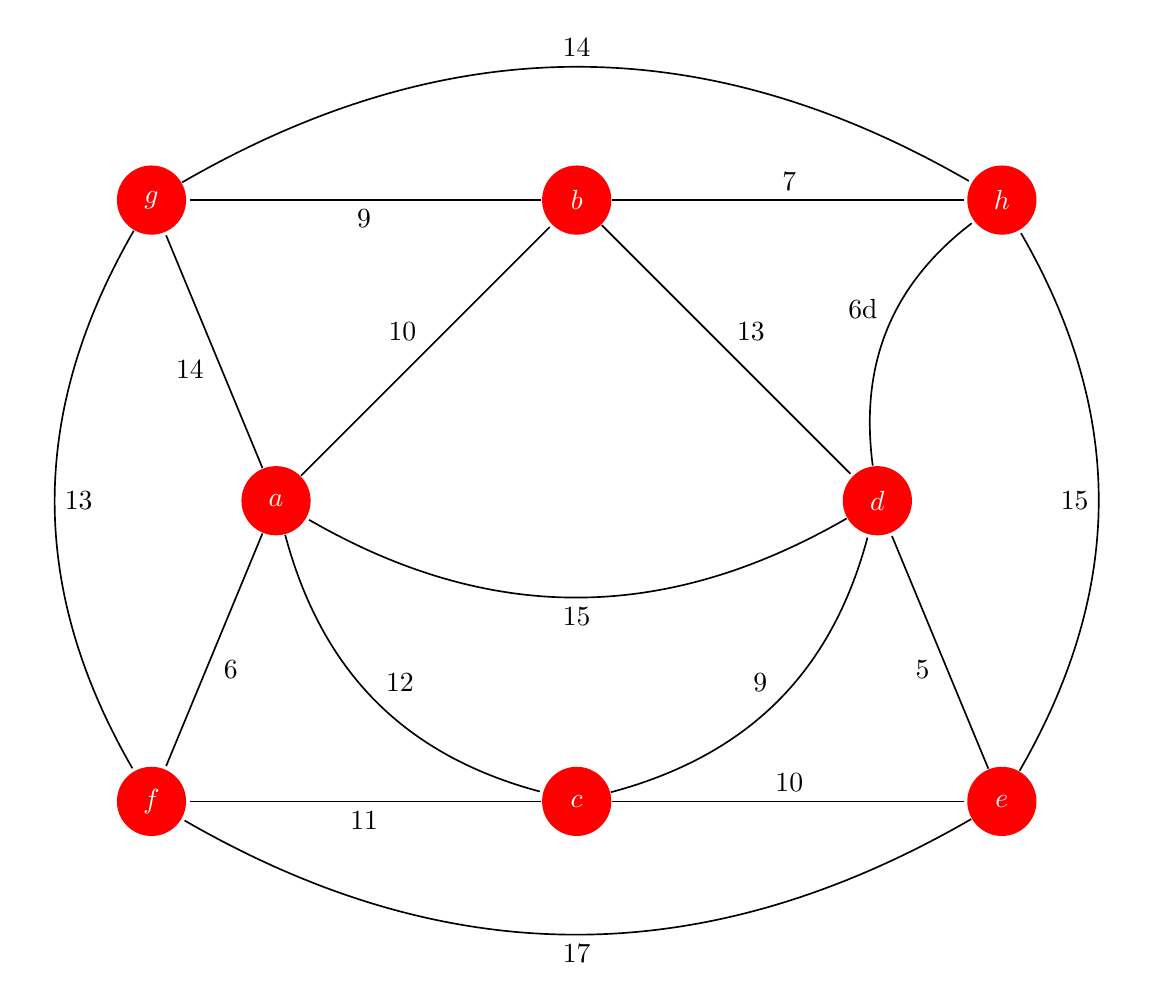
\begin{tikzpicture}[- ,shorten   >=1pt, auto, node distance=5.4cm, semithick]  %, >=stealth', 
  \tikzstyle{every state}=[fill=red,draw=none,text=white]
  \node[state] 	     (A)                             {$a$}; %initial,
  \node[state]         (B) [above right of=A] {$b$};
  \node[state]         (C) [below right of=A] {$c$};
  \node[state]         (D) [below right of=B] {$d$};
  \node[state]         (E) [right of= C]          {$e$};	
  \node[state]         (F) [ left of=C]          {$f$};
  \node[state]         (G) [left of=B]          {$g$};
  \node[state]         (H) [right of=B]          {$h$};
  \path (A) edge                 node  [auto] {10} (B)
            	edge                [bend right]  node [auto] {12} (C)
	           edge                node  [auto] {14} (G)
            	edge              node [auto] {6} (F)

         (B)   edge           node  [auto] {13} (D)
                 edge            node   [auto] {9} (G)
                 edge              node [auto] {7} (H)
                 
            (C) edge        [bend right]    node [auto] {9} (D)
                  edge               node [auto] {10} (E)
                  edge              node [auto] {11} (F)

 		(E)   edge      [bend right]        node  [auto] {15} (H)
               	         edge      [bend left]           node [auto] {17} (F)
		        edge               		         node [auto] {5} (D)
			
		(G)   edge      [bend right]           node [auto] {13} (F)
 		         edge      [bend left]              node [auto]  {14} (H)
			
			
       		 (D)   edge       [bend left]         node [auto] {15} (A)
       			edge          [bend left]        node [auto] {6d} (H);

\end{tikzpicture}\\

Using Kruskal's Algorithm:\\
1. $\{e, d\}$ W: 5 \\
2. $\{h, d\}$ W: 6 \\
3. $\{a, f\}$ W: 6 \\ 
4. $\{h, b\}$ W: 7 \\
5. $\{d, c\}$ W: 9 \\
6. $\{g, b\}$ W: 9 \\
7. $\{a, b\}$ W: 10 \\

\includegraphics[scale = 5]{DS1.png}\\

\eeq
\beq Describe the tree produced by breadth-first search and depth-first search for the n-cube graph $Q_n$, where n is a positive integer.\\

BFS:\\
Path of length $2^{n - 1 }$ that starts a vertex "v," and travels to all other vertices without forming a circle.\\

DFS:\\
It is a recursive tree that takes the original tree, $Q_{n - 1}$, and duplicates it. The trees are related by an edge, but does not have a cycle.\\

\eeq
\begin{q} \label{q:questao1} Build a binary search tree for the words: {\em oenology, phrenology, campanology, ornithology, ichthyology, limnology, alchemy,} and {\em astrology} using alphabetical order.

        \includegraphics[scale = 4]{DS2.png}\\

\end{q}\newpage
\begin{q}  For the tree in question \ref{q:questao1}  determine the order in which a inorder traversal visits the vertices of the given ordered rooted tree.\\

Astrology $->$ alchemy $->$ campanology $->$ limnology $->$ ichthyology $->$ oenology $->$ ornithology $->$ phrenology\\

\end{q}\newpage
\begin{q}  For the tree in question \ref{q:questao1}  determine the order in which a postorder traversal visits the vertices of the given ordered rooted tree.\\

Astrology $->$ alchemy $->$ limnology $->$ ichthyology $->$ campanology $->$ ornithology $->$ phrenology $->$ oenology\\

\end{q}\newpage
\begin{q} How many nonisomorphic unrooted trees are there with six vertices?\\

1. One with degree 2\\

2. Three with degree 3\\

3. One with degree 4\\

4. One with degree 5\\

Thus, there are 6 of them.\\

\end{q}\newpage
\begin{q} How many nonisomorphic rooted trees are there with six vertices?\\

1. One with height 5\\

2. Four with height 4\\

3. Eight with height 3\\

4. Six with height 2\\

5. One with height 1\\

Thus, there are 20 of them in all.\\

\end{q}\newpage
%%%questions
\end{document}
